\section{Instruzioni all'uso}
Tutte le funzionalità di HDViz sono facilmente reperibili ed nel menu laterale a scomparsa.

\subsection{Caricamento dati}
Inizialmente sono utilizzabili solo le prime voci:
\begin{itemize}
	\item Salva/Carica sessione;
	\item Carica dati dal database;
	\item Carica dati da \glo{CSV};
\end{itemize}
\begin{figure}[H]
		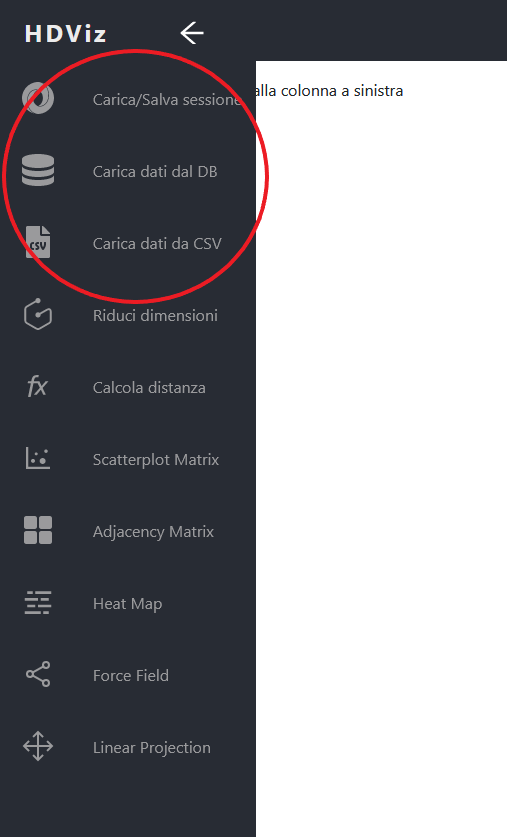
\includegraphics[scale=0.4]{Images/SceltaCaricamento.png}
		\centering
		\caption{Scelta del tipo di caricamento}
\end{figure}

Tutte e tre aprono una finestra di dialogo per compiere le operazioni indicate. In particolare:
\begin{itemize}
	\item La finestra per il caricamento dei dati dal database permette di scegliere uno dei dataset presenti nel database ed effettuare immediatamente una selezione delle dimensioni da caricare;
	\item  La finestra per il caricamento dei dati da file \glo{CSV} permette anche la selezione delle dimensioni che si desidera utilizzare (di default vengono utilizzate tutte quelle caricate)
	\begin{figure}[H]
		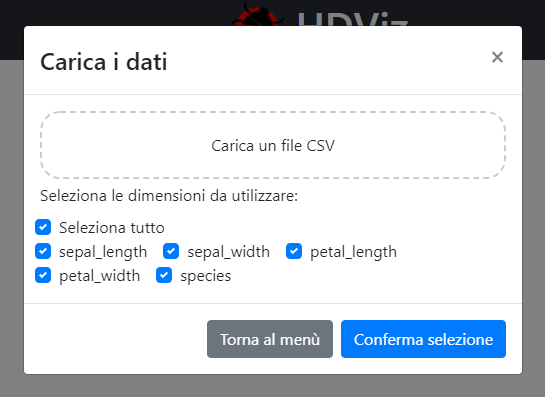
\includegraphics[scale=0.5]{Images/CaricamentoCSV.png}
		\centering
		\caption{Caricamento dati da file CSV}
	\end{figure}
\end{itemize}

Una volta caricati i dati è possibile selezionare anche tutte le altre voci del menu. Per la preparazione dei dati sono presenti le seguenti voci:

\begin{itemize}
	\item Riduci dimensioni;
	
	\item Calcola la distanza.
\end{itemize}

\begin{figure}[H]
		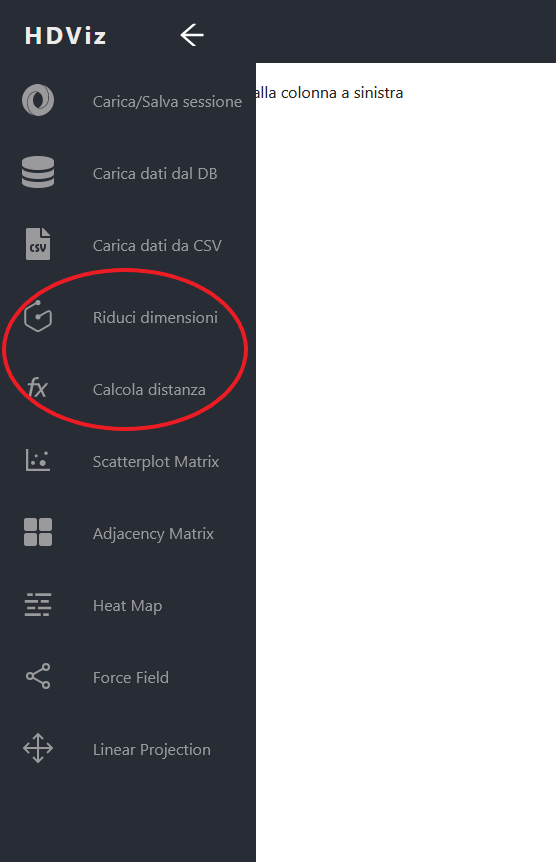
\includegraphics[scale=0.4]{Images/SceltaAlgoritmi.png}
		\centering
		\caption{Scelta dell'algoritmo}
\end{figure}

In ogni caso l'applicazione di algoritmi di riduzione dimensionale o funzioni per il calcolo della distanza \textbf{non sono obbligatori} per la visualizzazione dei dati. Se non si è interessati ai suddetti algoritmi si può passare direttamente a scegliere il grafico che più si preferisce tra quelli proposti.

\subsection{Riduzione dimensionale} 
Cliccando sulla voce "riduci dimensioni", si apre una finestra che permette di scegliere quali dimensioni utilizzare per la riduzione, quale algoritmo (tra \glo{Fastmap}, \glo{LLE}, \glo{Isomap} e \glo{TSNE}) e, in base a questa ultima scelta una serie di parametri per eseguire la riduzione come più si preferisce.
\begin{figure}[H]
		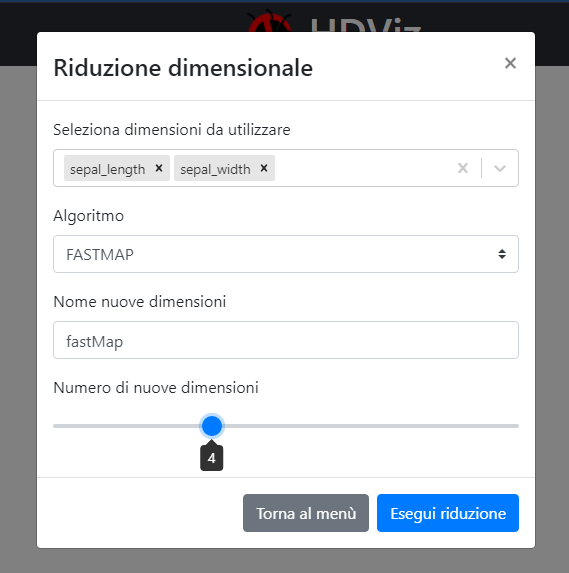
\includegraphics[scale=0.5]{Images/RiduzioneDimensionale.png}
		\centering
		\caption{Finestra per la riduzione dimensionale}
\end{figure}

\subsection{Calcolo della distanza}
Cliccando sulla voce "calcola distanza", si apre una finestra che permette di scegliere quali dimensioni utilizzare per effettuare il calcolo, quale funzione di distanza (tra Euclidea, Camberra, Chebyshev e Manhattan) e il nome da dare alla nuova matrice delle distanze creata.
\begin{figure}[H]
		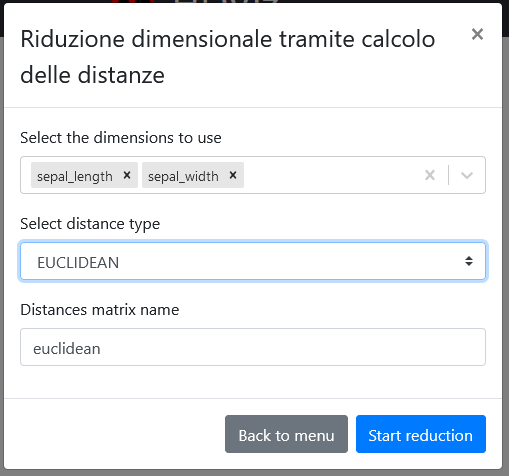
\includegraphics[scale=0.5]{Images/CalcoloDistanze.png}
		\centering
		\caption{Finestra per la riduzione dimensionale tramite il calcolo delle distanze}
\end{figure}

\subsection{Scelta del grafico e visualizzazione dei dati}
Una volta applicati gli algoritmi o meno, si può scegliere il grafico che più si preferisce tra quelli proposti:
\begin{itemize}
	\item \glo{Scatterplot Matrix};
	\item \glo{Adjency Matrix};
	\item \glo{Heat Map};
	\item \glo{Force Field};
	\item \glo{Linear Projection}.
\end{itemize}

\begin{figure}[H]
		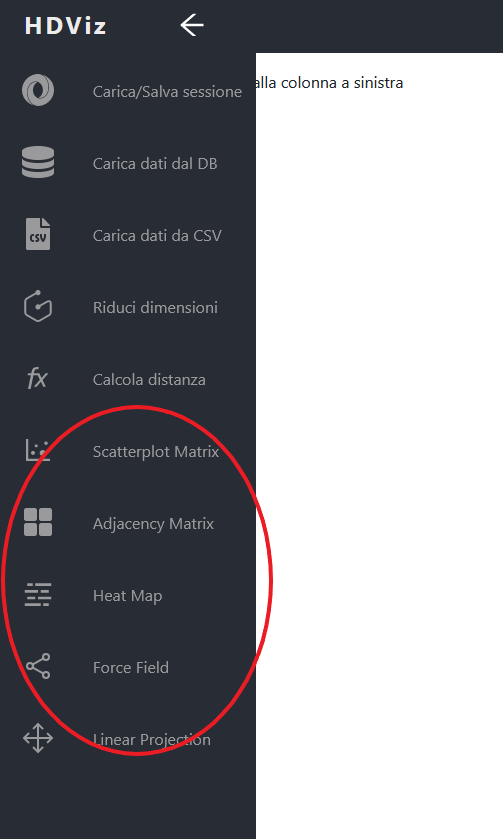
\includegraphics[scale=0.3]{Images/OptionList.png}
		\centering
		\caption{Lista dei grafici che è possibile scegliere}
\end{figure}

Una volta selezionata una di queste opzioni, si aprirà una \glo{form} sulla destra attraverso la quale sarà possibile modificare la visualizzazione del grafico.\\
Più precisamente la \glo{form} permette di:
\begin{itemize}
	\item Modificare le dimensioni da applicare agli assi;
	\item Modificare la dimensione per l'applicazione del colore sui punti;
	\item Modificare dimensioni per le visualizzazioni che ne fanno uso;
	\item Scegliere la matrice delle distanze da utilizzare tra quelle calcolate precedentemente (se sono state calcolate).
\end{itemize} 
Inizialmente tutti i campi siano settati a "No dimension". Tale \glo{form} è accompagnata da un bottone per nasconderla e centralizzare il grafico nello schermo per concentrarsi solamente sull'analisi del grafico.
\begin{figure}[H]
		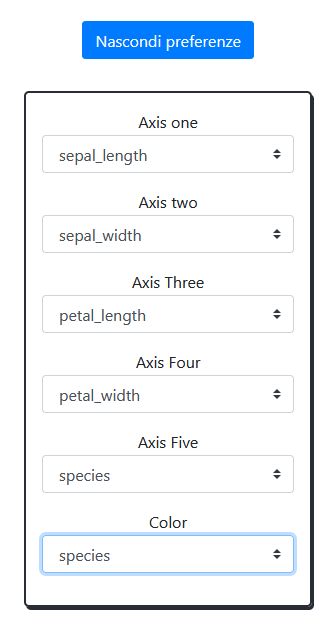
\includegraphics[scale=0.45]{Images/Form.png}
		\centering
		\caption{Esempio di form che appare dopo aver selezionato il tipo di grafico senza aver fatto scelto un algoritmo di riduzione dimensionale o calcolo delle distanze}
\end{figure}

\begin{figure}[H]
		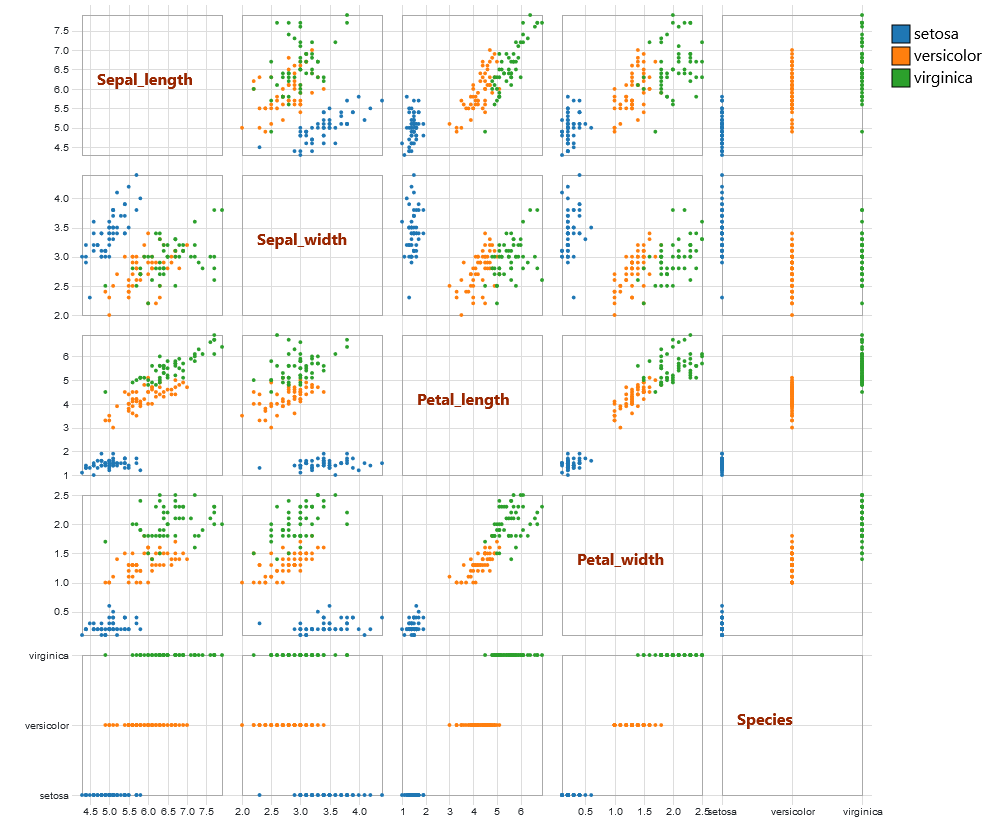
\includegraphics[scale=0.4]{Images/ScatterplotMatrix.png}
		\centering
		\caption{Esempio di visualizzazione dei dati nel caso si scegliesse lo Scatterplot Matrix e si riempissero tutti i campi della form sopra illustrata}
\end{figure}

